\documentclass[11pt,]{article}
\usepackage[left=1in,top=1in,right=1in,bottom=1in]{geometry}
\newcommand*{\authorfont}{\fontfamily{phv}\selectfont}
\usepackage[]{mathpazo}


  \usepackage[T1]{fontenc}
  \usepackage[utf8]{inputenc}




\usepackage{abstract}
\renewcommand{\abstractname}{}    % clear the title
\renewcommand{\absnamepos}{empty} % originally center

\renewenvironment{abstract}
 {{%
    \setlength{\leftmargin}{0mm}
    \setlength{\rightmargin}{\leftmargin}%
  }%
  \relax}
 {\endlist}

\makeatletter
\def\@maketitle{%
  \newpage
%  \null
%  \vskip 2em%
%  \begin{center}%
  \let \footnote \thanks
    {\fontsize{18}{20}\selectfont\raggedright  \setlength{\parindent}{0pt} \@title \par}%
}
%\fi
\makeatother




\setcounter{secnumdepth}{0}

\usepackage{longtable,booktabs}

\usepackage{graphicx,grffile}
\makeatletter
\def\maxwidth{\ifdim\Gin@nat@width>\linewidth\linewidth\else\Gin@nat@width\fi}
\def\maxheight{\ifdim\Gin@nat@height>\textheight\textheight\else\Gin@nat@height\fi}
\makeatother
% Scale images if necessary, so that they will not overflow the page
% margins by default, and it is still possible to overwrite the defaults
% using explicit options in \includegraphics[width, height, ...]{}
\setkeys{Gin}{width=\maxwidth,height=\maxheight,keepaspectratio}


\title{Making Migration Sexy: Immigrants in Same-Sex Couples in the United States  }



\author{\Large Nathan I. Hoffmann\vspace{0.05in} \newline\normalsize\emph{Department of Sociology, University of California, Los Angeles}   \and \Large Kristopher Velasco\vspace{0.05in} \newline\normalsize\emph{Departmnet of Sociology, University of Texas at Austin}  }


\date{}

\usepackage{titlesec}

\titleformat*{\section}{\normalsize\bfseries}
\titleformat*{\subsection}{\normalsize\itshape}
\titleformat*{\subsubsection}{\normalsize\itshape}
\titleformat*{\paragraph}{\normalsize\itshape}
\titleformat*{\subparagraph}{\normalsize\itshape}





\newtheorem{hypothesis}{Hypothesis}
\usepackage{setspace}


% set default figure placement to htbp
\makeatletter
\def\fps@figure{htbp}
\makeatother

\usepackage{fancyhdr}
\pagestyle{fancy}
\setlength{\headheight}{13.6pt}
\rhead{\textit{Hoffmann and Velasco}}

% move the hyperref stuff down here, after header-includes, to allow for - \usepackage{hyperref}

\makeatletter
\@ifpackageloaded{hyperref}{}{%
\ifxetex
  \PassOptionsToPackage{hyphens}{url}\usepackage[setpagesize=false, % page size defined by xetex
              unicode=false, % unicode breaks when used with xetex
              xetex]{hyperref}
\else
  \PassOptionsToPackage{hyphens}{url}\usepackage[draft,unicode=true]{hyperref}
\fi
}

\@ifpackageloaded{color}{
    \PassOptionsToPackage{usenames,dvipsnames}{color}
}{%
    \usepackage[usenames,dvipsnames]{color}
}
\makeatother
\hypersetup{breaklinks=true,
            bookmarks=true,
            pdfauthor={Nathan I. Hoffmann (Department of Sociology, University of California, Los Angeles) and Kristopher Velasco (Departmnet of Sociology, University of Texas at Austin)},
             pdfkeywords = {},  
            pdftitle={Making Migration Sexy: Immigrants in Same-Sex Couples in the United States},
            colorlinks=true,
            citecolor=blue,
            urlcolor=blue,
            linkcolor=blue,
            pdfborder={0 0 0}}
\urlstyle{same}  % don't use monospace font for urls

% Add an option for endnotes. -----


% add tightlist ----------
\providecommand{\tightlist}{%
\setlength{\itemsep}{0pt}\setlength{\parskip}{0pt}}

% add some other packages ----------

% \usepackage{multicol}
% This should regulate where figures float
% See: https://tex.stackexchange.com/questions/2275/keeping-tables-figures-close-to-where-they-are-mentioned
\usepackage[section]{placeins}


\begin{document}
	
% \pagenumbering{arabic}% resets `page` counter to 1 
%
% \maketitle

{% \usefont{T1}{pnc}{m}{n}
\setlength{\parindent}{0pt}
\thispagestyle{plain}
{\fontsize{18}{20}\selectfont\raggedright 
\maketitle  % title \par  

}

{
   \vskip 13.5pt\relax \normalsize\fontsize{11}{12} 
\textbf{\authorfont Nathan I. Hoffmann} \hskip 15pt \emph{\small Department of Sociology, University of California, Los Angeles}   \par \textbf{\authorfont Kristopher Velasco} \hskip 15pt \emph{\small Departmnet of Sociology, University of Texas at Austin}   

}

}






\vskip -8.5pt


 % removetitleabstract

\noindent  

\hypertarget{data}{%
\section{Data}\label{data}}

We merge individual-level data on immigrants in the U.S. with state- and country-level variables from a variety of datasets. The individual data come from the 2008 to 2019 American Community Survey (ACS). Each year, the ACS surveys a 1\% sample of the U.S. population about their education, occupation, income, family structure, immigration status, country of origin, location, and a variety of other individual and household attributes. Although the ACS began in 2000, variables on same-sex partners were not reliable until 2008 (U.S. Census Bureau \protect\hyperlink{ref-u.s.censusbureau_2013}{2013}). We limit the sample to individuals who immigrated at the age of 18 or older. The 11 years of survey data contain 9,325 same-sex couples that include at least one immigrant, for a total of 12,443 immigrants in same-sex couples. These immigrants are compared to 985,884 corresponding different-sex couples (containing 1,626,731 individual immigrants).

Our explanatory variables of interest are the LGBT policy context in country of origin and U.S. state of residence. To create the U.S. state policy index, we compile data from the Movement Advancement Project, a leading LGBT organization in the U.S. that collects data on a number of relevant policies. Our state index encompasses both progressive policies (full marriage equality, state recognition of civil unions and domestic partnerships, ban on all employment and housing discrimination based on sexual orientation, hate crime protections based on sexual orientation, legal joint adoption by same-sex couples, and a ban on conversation therapy for minors) and regressive policies (criminalization of sodomy, state constitutional bans of marriage equality, religious freedom exemptions to discriminate against same-sex couples in adoption, and state-level bans on local non-discrimination ordinances encompassing sexual orientation). The state index ranges from -2 to 7, and the mean score of country of origin for immigrant in our sample is 3.2.

We measure the origin country policy environment using the LGBT Policy Index (Velasco \protect\hyperlink{ref-velasco_2018}{2018}). This index comprises 14 policies, many similar to those above, but including additional policies like the death penalty for homosexual acts, propaganda laws limiting free speech for LGBT communities, and equal age of consent between same-sex and opposite-sex couples. Both indices are created by summing the net total of progressive policies (scored +1) over regressive policies (scored -1). The state index ranges from -3.2 to 11, and the mean score of country of origin for immigrant in our sample is 1.7.

Immigrants are assigned state index scores (destination policy environment) based on their self-reported state of residence during the year of the ACS survey. They are assigned country index scores (origin policy environment) based on their year of immigration. Since the country policy index begins at 1991, we anyone who immigrated before 1991 gets assigned the 1991 value.

Our country- and state-level controls come from a variety of sources. Country-of-origin controls for bilateral distance, contiguous border, common official language, common ethnic language, and whether the country was a former colony of the U.S. come from CEPII's GeoDist dataset. Difference in wages (in 1000s of 2011 US dollars) come from the Penn World Table, and we rely on World Bank data for differences in unemployment rates. We use Polity5 measures of democratization of the country of origin. For state controls, we use per capita income by year from the Bureau of Economic Analysis and state-level annual unemployment rates from the Bureau of Labor Statistics.

For our individual-level analysis we include individual controls from the ACS for reported sex, age, education (with categories for less than high school, high school, some college, and college), log positive income, and a binary indicator for income reported to be 0 or less.

\hypertarget{analytic-strategy}{%
\section{Analytic Strategy}\label{analytic-strategy}}

Our first goal is to isolate the effects of country-of-origin LGBT policy on the immigration of immigrants in same-sex couples. The ideal survey would follow potential immigrants over time and have information about sexual orientation, allowing us to estimate how the probability of migrating and choice of U.S. state of residence vary by sexual orientation. This ideal dataset does not exist, but we approximate it at the macro level. We take the number of immigrants in same-sex couples from a given country and a given year of immigration and divide by the total number of immigrants from that country-year. If sending-country LGBT policy has no effect on migration rates of LGB immigrants, then we would expect these proportions to be similar between countries. However, LGBT policy may covary with potential confounders such as country income, unemployment, democratization, and relationship to the U.S., so we control for these variables in our preferred model and estimate using ordinary least squares (OLS) regression. We also specify models with country fixed or random effects to account for unobserved heterogeneity within countries. All of these models also have country-clustered standard errors.

Our next set of models focus on U.S. state LGBT policy. We reshape the data so that each observation is the proportion of immigrants in same-sex couples from country \(x\) in state \(y\) in year \(z\). We regress this proportion on state and sending-country policy scores, controlling for the same country- and state-level attributes as in the previous set of models. We include state and country-of-origin fixed effects, and cluster errors at the state level.

Our final set of models turns toward the individual: conditional on immigrating to the U.S., do immigrant in same-sex couples choose more LGBT-friendly states to reside in? This part of the analysis uses ordered logistic regression to predict the policy index of state of residence. Whereas the full U.S. state policy index ranges from -2 to \texttt{max(acs\_couple\_policy\$state\_policy,\ na.rm\ =\ T)}, we break up the index into three ``bins'': repressive (0 and less), neutral (1 or 2), and progressive (3 and greater). We control for individual attributes that could possibly confound our results and include survey-year fixed effects and country-clustered standard errors.

\hypertarget{results}{%
\section{Results}\label{results}}

\hypertarget{descriptive-statistics}{%
\subsection{Descriptive statistics}\label{descriptive-statistics}}

We first estimate total numbers of immigrants in same- and different-sex couples, applying survey weights to obtain population-level estimates from the ACS. Figure \ref{fig:toal-pop} shows that whereas numbers of different-sex immigrant couples have steadily increased over the period of study, numbers of same-sex immigrant couples have increased much more rapidly, especially since the the 2013 Supreme Court decision overturning DOMA.

Figure \ref{fig:policy-desc} charts the average country-of-origin and U.S.-state policy score for the immigrants in our sample over time, comparing means for immigrants in same- and different-sex couples. The left panel shows that country-of-origin index at time of migration is generally higher for immigrants in same-sex couples, especially in recent years. Immigrants in same-sex couples tend to come from more progressive countries. The left panel indicates less of a difference in U.S. state policies, although states where immigrants in same-sex couples tend to score somewhat higher.

\begin{figure}
\centering
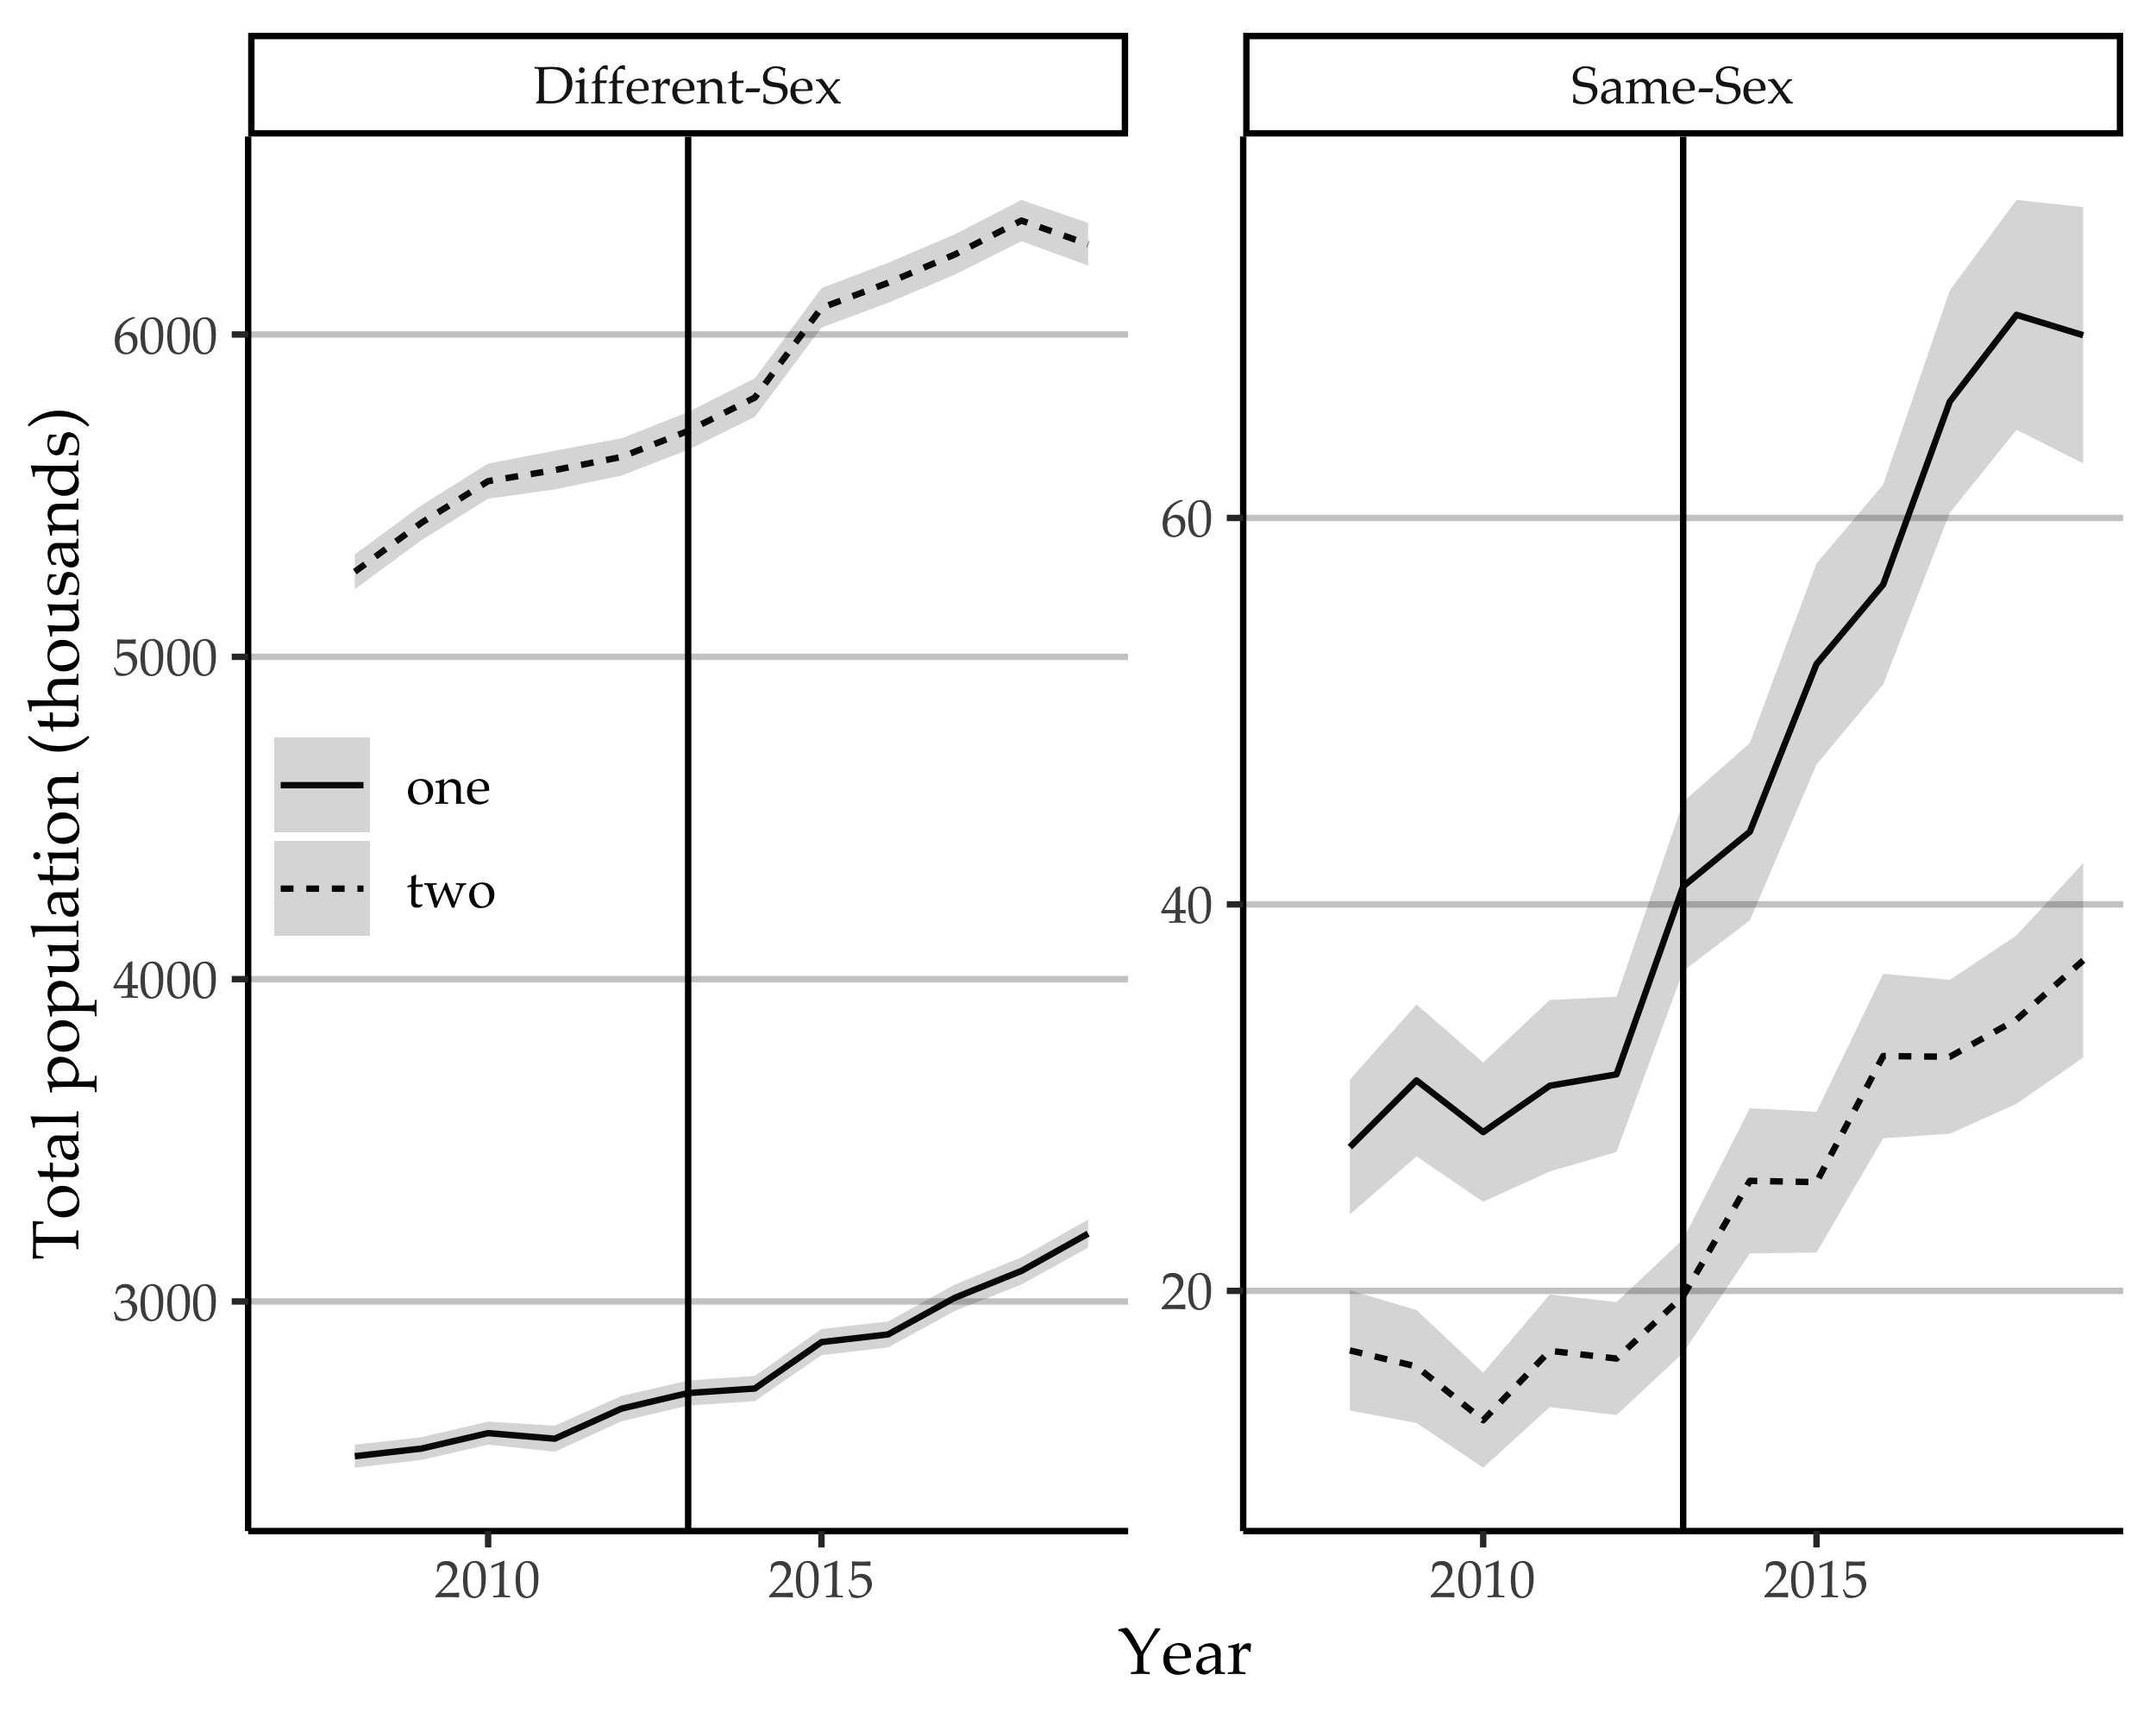
\includegraphics{ssimm_draft_methods_results_files/figure-latex/total-pop-1.pdf}
\caption{\label{fig:total-pop}Estimated totals of different- and same-sex couples containing one or two immigrants, 2008-2019, with 95\% confidence intervals. Vertical line placed at the year 2013, when DOMA was overturned.}
\end{figure}

\begin{figure}
\centering
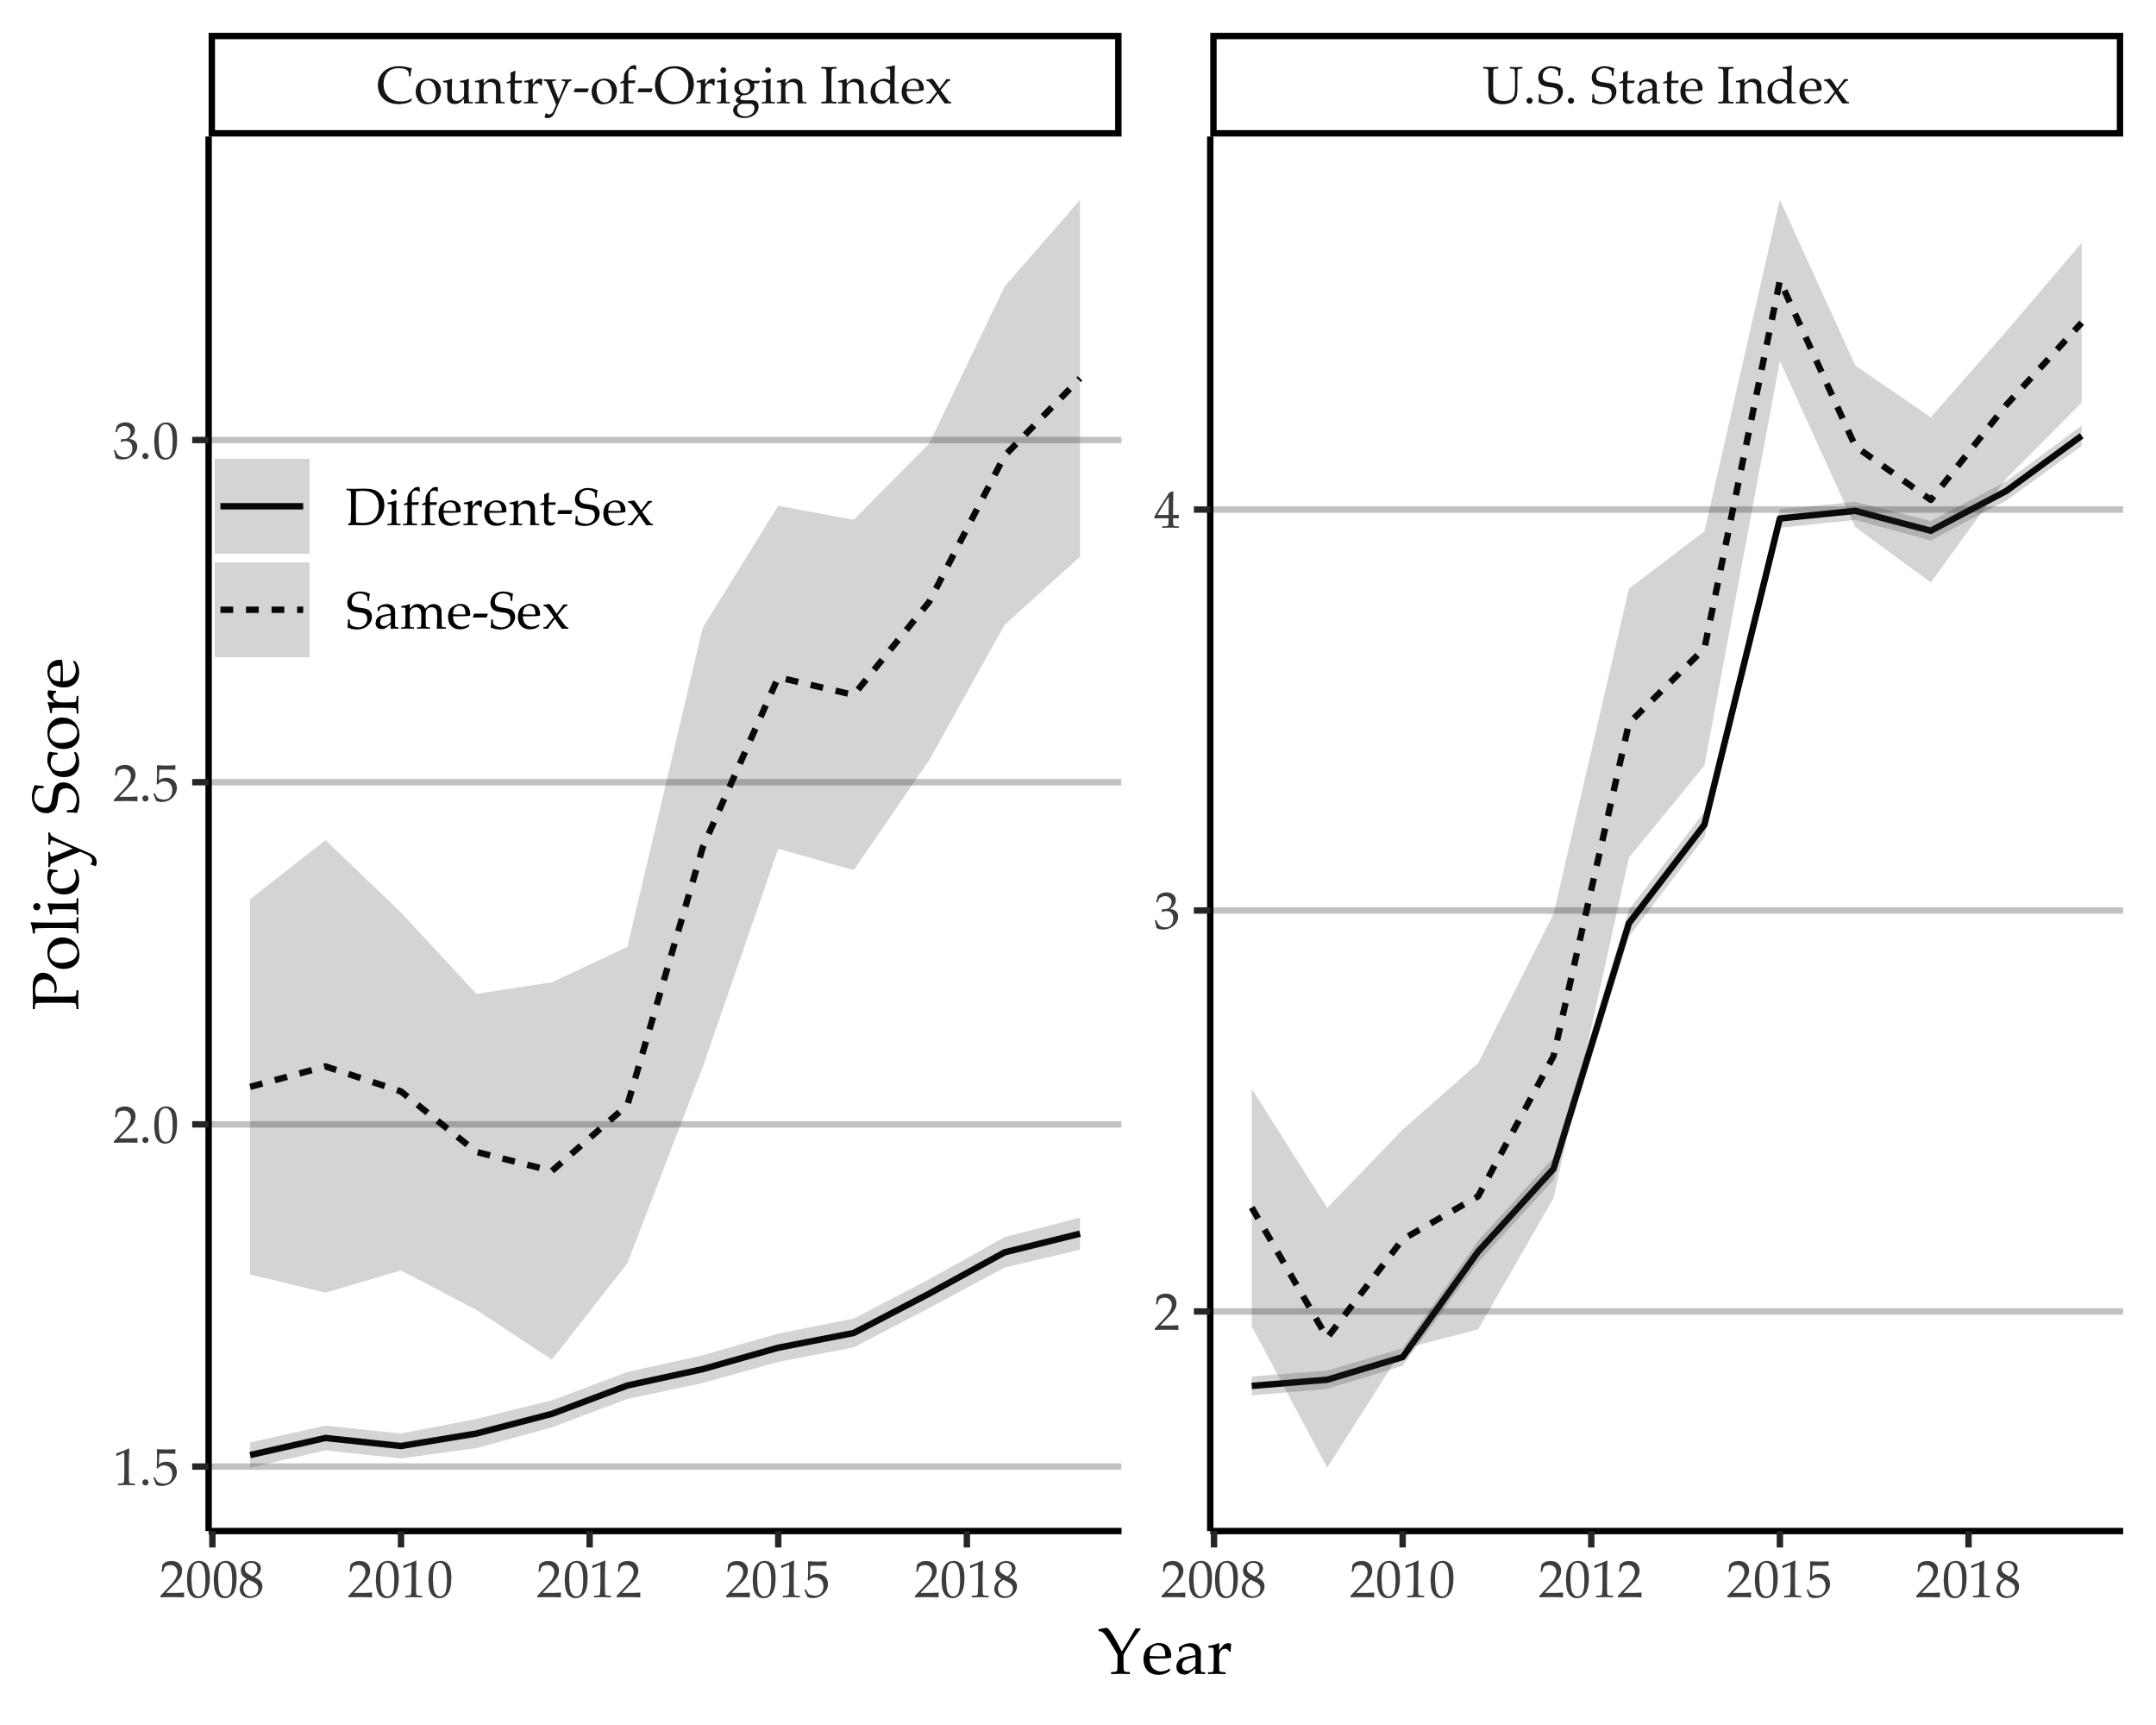
\includegraphics{ssimm_draft_methods_results_files/figure-latex/policy-desc-1.pdf}
\caption{\label{fig:policy-desc}Mean country-of-origin and U.S. state policy index score for immigrants in same- and different-sex couples, 2008-2019, with 95\% confidence intervals.}
\end{figure}

\begin{table}

\caption{\label{tab:country-tab}Sending countries ranked bby proportion immigrant couples with same-sex partners}
\centering
\begin{tabular}[t]{lllr}
\toprule
Rank & Country of origin & Proportion same-sex & Average policy score\\
\midrule
1 & Australia & 2.53 \% & 4.08\\
2 & Mongolia & 2.37 \% & 2.25\\
3 & Belgium & 2.25 \% & 4.98\\
4 & New Zealand & 2.12 \% & 5.43\\
5 & Singapore & 2.11 \% & -0.20\\
6 & Netherlands & 2.08 \% & 7.15\\
7 & France & 2.05 \% & 6.07\\
8 & Malaysia & 2.05 \% & -0.89\\
9 & Zimbabwe & 2.01 \% & -0.95\\
10 & Spain & 1.98 \% & 5.60\\
\bottomrule
\end{tabular}
\end{table}

\begin{table}

\caption{\label{tab:state-tab}States ranked by proportion immigrant couples with same-sex partners}
\centering
\begin{tabular}[t]{lllr}
\toprule
Rank & State & Proportion same-sex & Mean policy score\\
\midrule
1 & Vermont & 2.09 \% & 5.17\\
2 & Maine & 1.63 \% & 4.79\\
3 & Montana & 1.47 \% & 0.81\\
4 & Missouri & 1.18 \% & 1.91\\
5 & Massachusetts & 1.12 \% & 4.77\\
6 & New York & 1.10 \% & 4.84\\
7 & Florida & 1.01 \% & 0.91\\
8 & Mississippi & 1.00 \% & -0.49\\
9 & Minnesota & 0.96 \% & 4.63\\
10 & New Hampshire & 0.95 \% & 4.33\\
\bottomrule
\end{tabular}
\end{table}

Table \ref{tab:country-tab} ranks the proportion of U.S. immigrants in same-sex couples based on country of origin, averaging over the 11 years of survey data. The top sending countries show a mix of progressive and repressive policies. For example, Australia has a score of 4.1, indicating rather progressive policies, and Mongolia's are somewhat progressive at 0. But Malaysia and Zimbabwe exhibit generally repressive policies at the year of departure of the immigrants in our sample, with average scores of -0.89 and -0.95, respectively.

Table \ref{tab:state-tab} similarly ranks by U.S. state the proportion of immigrants in same-sex couples, averaging over the period of interest. Although states with progressive policies make the top of the list (e.g.~Vermont's average score is 5.2), states with more repressive policies also figure in to the top 10, such as Mississippi with -0.49.

\hypertarget{models}{%
\subsection{Models}\label{models}}

\begin{table}[!htbp] \centering 
  \caption{100*Proportion same-sex in a country-year of immigration} 
  \label{tab:country-props} 
\begin{tabular}{@{\extracolsep{5pt}}lccccc} 
\\[-1.8ex]\hline 
\hline \\[-1.8ex] 
 & \multicolumn{5}{c}{\textit{Dependent variable:}} \\ 
\cline{2-6} 
\\[-1.8ex] & \multicolumn{5}{c}{prop\_same\_sex} \\ 
\\[-1.8ex] & (1) & (2) & (3) & (4) & (5)\\ 
\hline \\[-1.8ex] 
 origin\_score & 0.079$^{***}$ &  & 0.066$^{***}$ & 0.037$^{+}$ & 0.062$^{***}$ \\ 
  & (0.007) &  & (0.010) & (0.019) & (0.013) \\ 
  & & & & & \\ 
 distw &  & 0.00002$^{*}$ & 0.00003$^{**}$ & 0.002$^{*}$ & 0.00003$^{+}$ \\ 
  &  & (0.00001) & (0.00001) & (0.001) & (0.00001) \\ 
  & & & & & \\ 
 contig &  & 0.110 & $-$0.037 & 2.500$^{+}$ & $-$0.039 \\ 
  &  & (0.200) & (0.200) & (1.500) & (0.290) \\ 
  & & & & & \\ 
 comlang\_off &  & $-$0.012 & 0.003 & $-$17.000$^{*}$ & 0.006 \\ 
  &  & (0.081) & (0.081) & (7.900) & (0.120) \\ 
  & & & & & \\ 
 comlang\_ethno &  & $-$0.051 & 0.010 & 8.500$^{*}$ & 0.001 \\ 
  &  & (0.069) & (0.069) & (3.800) & (0.100) \\ 
  & & & & & \\ 
 colony &  & 0.300$^{*}$ & 0.120 & 12.000$^{*}$ & 0.150 \\ 
  &  & (0.140) & (0.140) & (5.700) & (0.200) \\ 
  & & & & & \\ 
 wage\_dif &  & 0.00001 & $-$0.00001 & 0.00001 & $-$0.00000 \\ 
  &  & (0.00001) & (0.00001) & (0.00001) & (0.00001) \\ 
  & & & & & \\ 
 unemp\_dif &  & $-$0.002 & $-$0.002 & 0.005 & $-$0.0005 \\ 
  &  & (0.004) & (0.004) & (0.009) & (0.005) \\ 
  & & & & & \\ 
 polity5 &  & 0.036$^{***}$ & 0.023$^{***}$ & 0.0004 & 0.020$^{***}$ \\ 
  &  & (0.004) & (0.005) & (0.010) & (0.006) \\ 
  & & & & & \\ 
\hline \\[-1.8ex] 
Country-clustered SEs? & yes & yes & yes & yes & NA \\ 
Country FEs? & no & no & no & yes & no \\ 
Country REs? & no & no & no & no & yes \\ 
Observations & 3,811 & 2,995 & 2,995 & 2,995 & 2,995 \\ 
R$^{2}$ & 0.031 & 0.028 & 0.041 & 0.120 &  \\ 
\hline 
\hline \\[-1.8ex] 
\textit{Note:}  & \multicolumn{5}{r}{+p<0.1; *p<0.05; **p<0.01; ***p<0.001} \\ 
\end{tabular} 
\end{table}

\begin{table}[!htbp] \centering 
  \caption{100*Proportion same-sex in a country-state-year} 
  \label{tab:state-props} 
\begin{tabular}{@{\extracolsep{5pt}}lccc} 
\\[-1.8ex]\hline 
\hline \\[-1.8ex] 
 & \multicolumn{3}{c}{\textit{Dependent variable:}} \\ 
\cline{2-4} 
\\[-1.8ex] & \multicolumn{3}{c}{same\_prop} \\ 
\\[-1.8ex] & (1) & (2) & (3)\\ 
\hline \\[-1.8ex] 
 state\_unemploy &  & $-$0.033$^{+}$ & $-$0.001 \\ 
  &  & (0.017) & (0.023) \\ 
  & & & \\ 
 state\_income &  & 0.00001 & $-$0.00003 \\ 
  &  & (0.00001) & (0.00002) \\ 
  & & & \\ 
 origin\_score & 0.053$^{***}$ & 0.050$^{***}$ & 0.110$^{**}$ \\ 
  & (0.011) & (0.011) & (0.040) \\ 
  & & & \\ 
 distw &  &  & 0.004$^{***}$ \\ 
  &  &  & (0.001) \\ 
  & & & \\ 
 contig &  &  & 5.900$^{***}$ \\ 
  &  &  & (1.600) \\ 
  & & & \\ 
 comlang\_off &  &  & $-$35.000$^{***}$ \\ 
  &  &  & (8.600) \\ 
  & & & \\ 
 comlang\_ethno &  &  & 18.000$^{***}$ \\ 
  &  &  & (4.100) \\ 
  & & & \\ 
 colony &  &  & 26.000$^{***}$ \\ 
  &  &  & (6.200) \\ 
  & & & \\ 
 wage\_dif &  &  & 0.0001$^{**}$ \\ 
  &  &  & (0.0001) \\ 
  & & & \\ 
 unemp\_dif &  &  & $-$0.022$^{+}$ \\ 
  &  &  & (0.012) \\ 
  & & & \\ 
 polity5 &  &  & $-$0.001 \\ 
  &  &  & (0.012) \\ 
  & & & \\ 
 state\_policy & 0.033$^{+}$ & 0.008 & 0.041 \\ 
  & (0.017) & (0.034) & (0.036) \\ 
  & & & \\ 
\hline \\[-1.8ex] 
State-clustered SEs? & yes & yes & yes \\ 
State FEs? & no & yes & yes \\ 
Country FEs? & no & no & yes \\ 
Observations & 44,431 & 44,076 & 39,147 \\ 
R$^{2}$ & 0.001 & 0.003 & 0.010 \\ 
\hline 
\hline \\[-1.8ex] 
\textit{Note:}  & \multicolumn{3}{r}{+p<0.1; *p<0.05; **p<0.01; ***p<0.001} \\ 
\end{tabular} 
\end{table}

\begin{table}[!htbp] \centering 
  \caption{Individual ordered logit analysis of three-category state policy score} 
  \label{tab:ord} 
\begin{tabular}{@{\extracolsep{5pt}}lccc} 
\\[-1.8ex]\hline 
\hline \\[-1.8ex] 
 & \multicolumn{3}{c}{\textit{Dependent variable:}} \\ 
\cline{2-4} 
\\[-1.8ex] & \multicolumn{3}{c}{state\_policy\_binned} \\ 
\\[-1.8ex] & (1) & (2) & (3)\\ 
\hline \\[-1.8ex] 
 same\_sex & 0.210$^{***}$ & 0.140$^{***}$ & 26.000$^{***}$ \\ 
  & (0.002) & (0.003) & (0.00003) \\ 
  origin\_score &  & $-$0.047$^{***}$ & $-$0.019$^{***}$ \\ 
  &  & (0.0003) & (0.0003) \\ 
  sexMale &  &  & $-$0.093$^{***}$ \\ 
  &  &  & (0.001) \\ 
  age &  &  & 0.002$^{***}$ \\ 
  &  &  & (0.0001) \\ 
  educcollege &  &  & 0.076$^{***}$ \\ 
  &  &  & (0.002) \\ 
  educHS &  &  & $-$0.010$^{***}$ \\ 
  &  &  & (0.002) \\ 
  educsome col &  &  & 0.0001 \\ 
  &  &  & (0.002) \\ 
  nchild &  &  & 0.023$^{***}$ \\ 
  &  &  & (0.001) \\ 
  log\_income &  &  & 0.074$^{***}$ \\ 
  &  &  & (0.0002) \\ 
  no\_income &  &  & 0.640$^{***}$ \\ 
  &  &  & (0.0002) \\ 
  yrimmig &  &  & $-$0.019$^{***}$ \\ 
  &  &  & (0.00000) \\ 
  same\_sexTRUE:origin\_score &  & 0.042$^{***}$ & 0.056$^{***}$ \\ 
  &  & (0.001) & (0.001) \\ 
  same\_sexTRUE:sexMale &  &  & 0.110$^{***}$ \\ 
  &  &  & (0.0002) \\ 
  same\_sexTRUE:age &  &  & $-$0.007$^{***}$ \\ 
  &  &  & (0.0002) \\ 
  same\_sexTRUE:educcollege &  &  & 0.091$^{***}$ \\ 
  &  &  & (0.0003) \\ 
  same\_sexTRUE:educHS &  &  & $-$0.028$^{***}$ \\ 
  &  &  & (0.0002) \\ 
  same\_sexTRUE:educsome col &  &  & 0.075$^{***}$ \\ 
  &  &  & (0.0002) \\ 
  same\_sexTRUE:nchild &  &  & $-$0.030$^{***}$ \\ 
  &  &  & (0.002) \\ 
  same\_sexTRUE:log\_income &  &  & 0.030$^{***}$ \\ 
  &  &  & (0.001) \\ 
  same\_sexTRUE:no\_income &  &  & 0.390$^{***}$ \\ 
  &  &  & (0.0001) \\ 
  same\_sexTRUE:yrimmig &  &  & $-$0.013$^{***}$ \\ 
  &  &  & (0.00001) \\ 
 \hline \\[-1.8ex] 
Country-clustered SEs? & yes & yes & yes \\ 
Survey year FEs? & yes & yes & yes \\ 
Observations & 11,811,332 & 11,321,972 & 11,321,972 \\ 
\hline 
\hline \\[-1.8ex] 
\textit{Note:}  & \multicolumn{3}{r}{+p<0.1; *p<0.05; **p<0.01; ***p<0.001} \\ 
\end{tabular} 
\end{table}

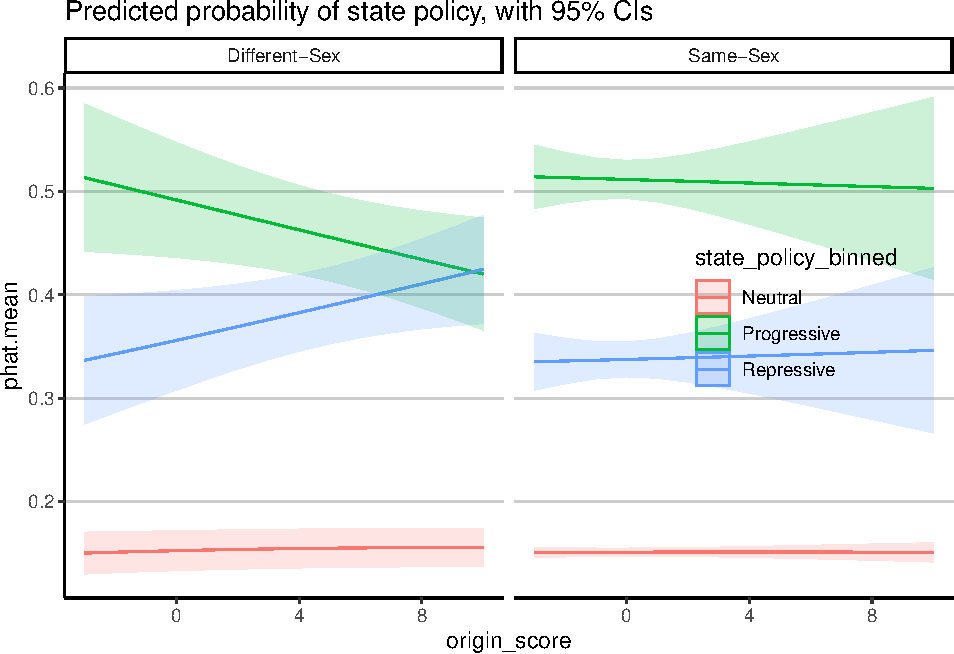
\includegraphics{ssimm_draft_methods_results_files/figure-latex/sim-1.pdf}

\hypertarget{references}{%
\section{References}\label{references}}

\setlength{\parindent}{-0.2in}
\setlength{\leftskip}{0.2in}
\setlength{\parskip}{8pt}

\noindent

\hypertarget{refs}{}
\leavevmode\hypertarget{ref-u.s.censusbureau_2013}{}%
U.S. Census Bureau. 2013. ``Frequently Asked Questions About Same-Sex Couple Households.'' U.S. Census Bureau Fertility; Family STatistics Branch.

\leavevmode\hypertarget{ref-velasco_2018}{}%
Velasco, Kristopher. 2018. ``Human Rights INGOs, LGBT INGOs, and LGBT Policy Diffusion, 1991--2015.'' \emph{Social Forces} 97 (1): 377--404. \url{https://doi.org/10.1093/sf/soy030}.

\newpage
\singlespacing 
\end{document}
